\section{Presentation Logic Layer}

%What pages will be present in your project? briefly indicate how your web site will be organized

Lorem ipsum dolor sit amet, consectetur adipiscing elit, sed do eiusmod tempor incididunt ut labore et dolore magna aliqua. Ut enim ad minim veniam, quis nostrud exercitation ullamco laboris nisi ut aliquip ex ea commodo consequat. Duis aute irure dolor in reprehenderit in voluptate velit esse cillum dolore eu fugiat nulla pariatur. Excepteur sint occaecat cupidatat non proident, sunt in culpa qui officia deserunt mollit anim id est laborum.

\subsection{Signup page}

\begin{center}
	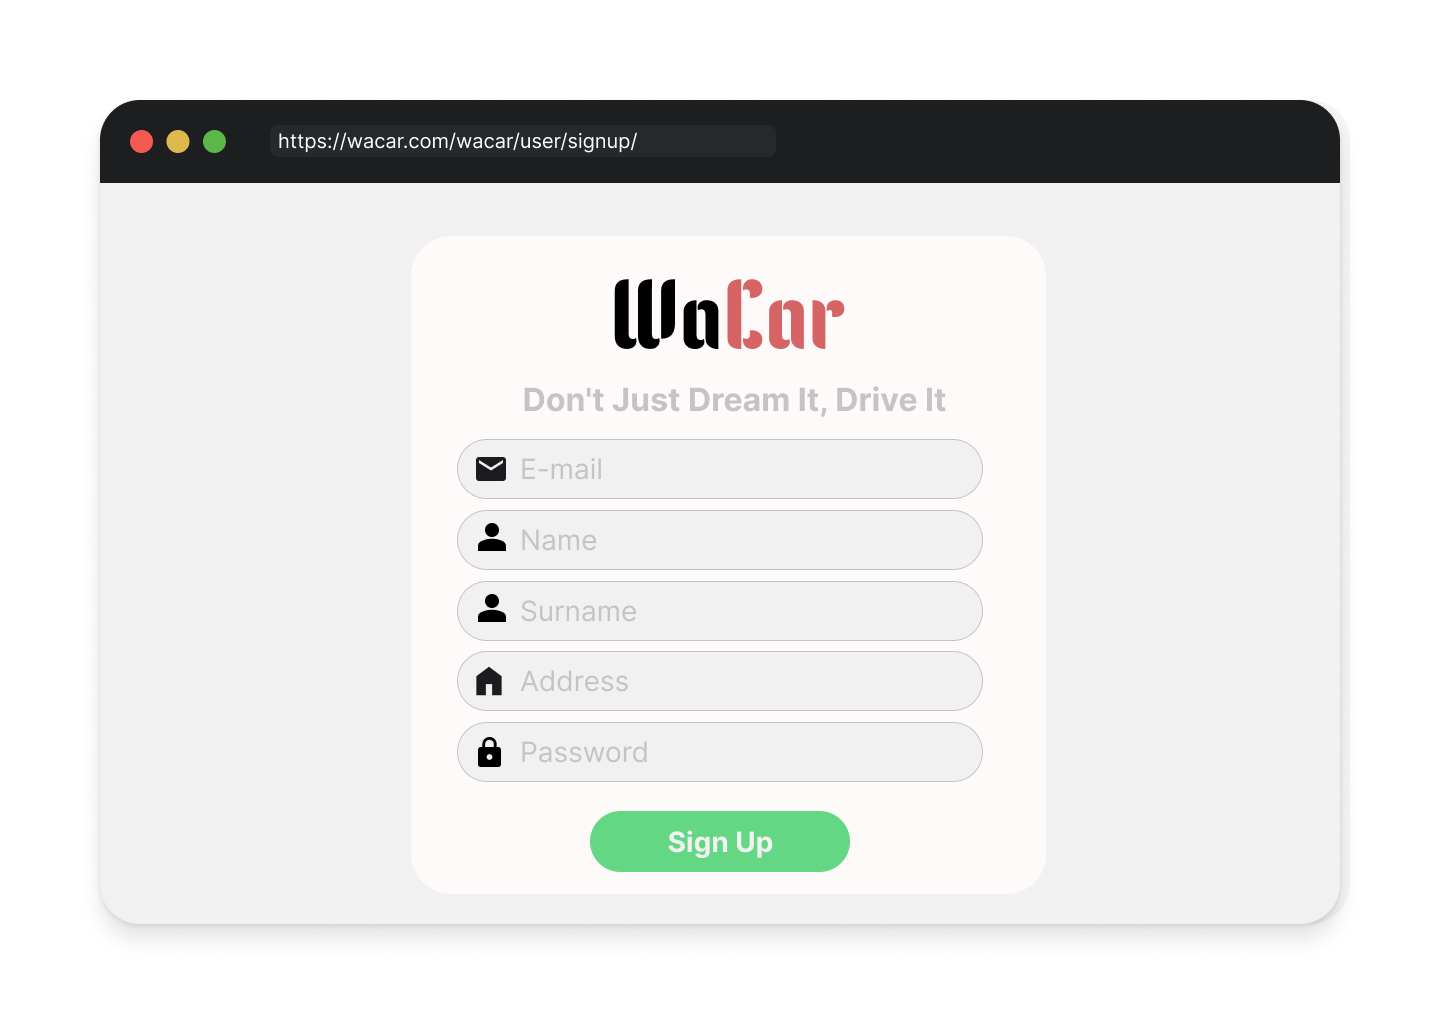
\includegraphics[scale=0.3]{./mockup/signUp.png}
	\captionof{figure}{WACAR SignUp page}
	\label{ERSchema}
\end{center}


On the Signup page, users can input their credentials to gain access to the order page, user information page, as well as a list of past orders.
The required information includes email, password, name, surname, and address. The password must meet certain criteria, including a minimum of 8 characters, at least one number, and at least one uppercase letter. 
Upon clicking "Signup" the user's credentials are added to the database, and they are redirected to the homepage.
If the provided credentials do not meet the required criteria an error message is displayed to the user.
The login process mirrors the signup process, but only requires the user to input their email and password. Upon clicking "Login" a search is conducted in the database. 
If the provided email exists and the user's password matches the encrypted password stored in the database, the login operation is executed, otherwise the user is informed that email or password are incorrect.

\subsection{Homepage}

\begin{center}
	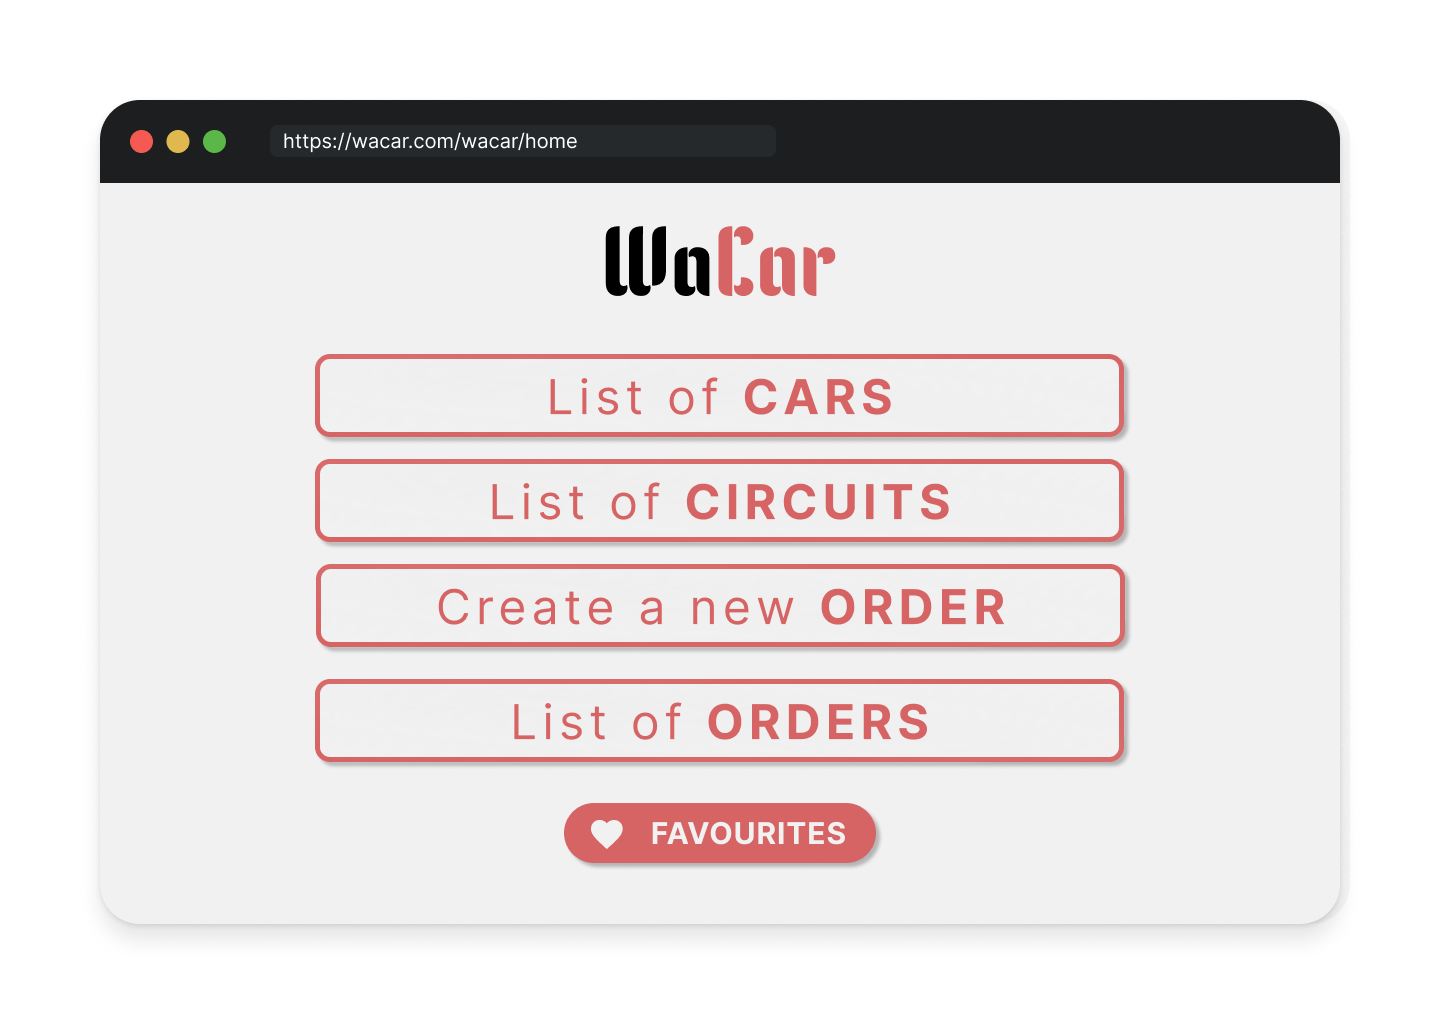
\includegraphics[scale=0.3]{./mockup/user_home.png}
	\captionof{figure}{WACAR Homepage}
	\label{ERSchema}
\end{center}

The homepage serves as the initial landing point for users upon opening WaCar. Its content dynamically adapts to the session state: when user is not logged in, 
they encounter two cards displaying options to explore available cars and circuits. Additionally, login and signup buttons are provided.
If the user is logged in, in addition to the previously mentioned cards, ordering cards will also appear, enabling them to create new orders, as well as the user page.

If an admin accesses the page instead of a regular user, distinct cards are presented, allowing them to add, edit and remove cars and circuits from the database.

\subsection{CarList}

\begin{center}
	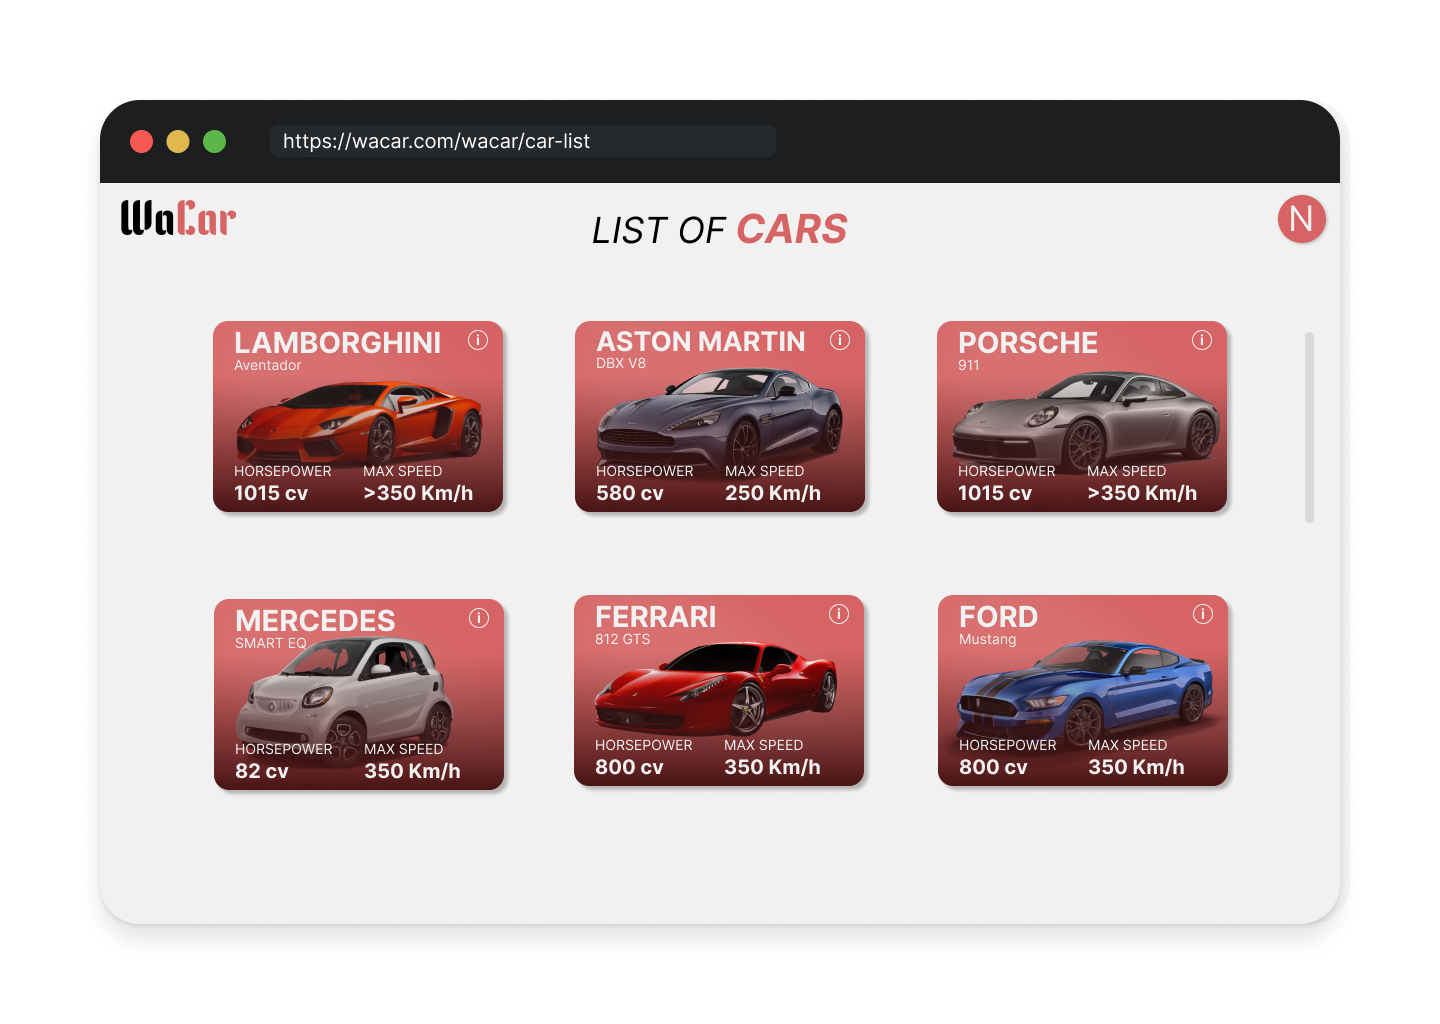
\includegraphics[scale=0.3]{./mockup/car_list.png}
	\captionof{figure}{WACAR car list}
	\label{ERSchema}
\end{center}

\subsection{Order page}

\begin{center}
	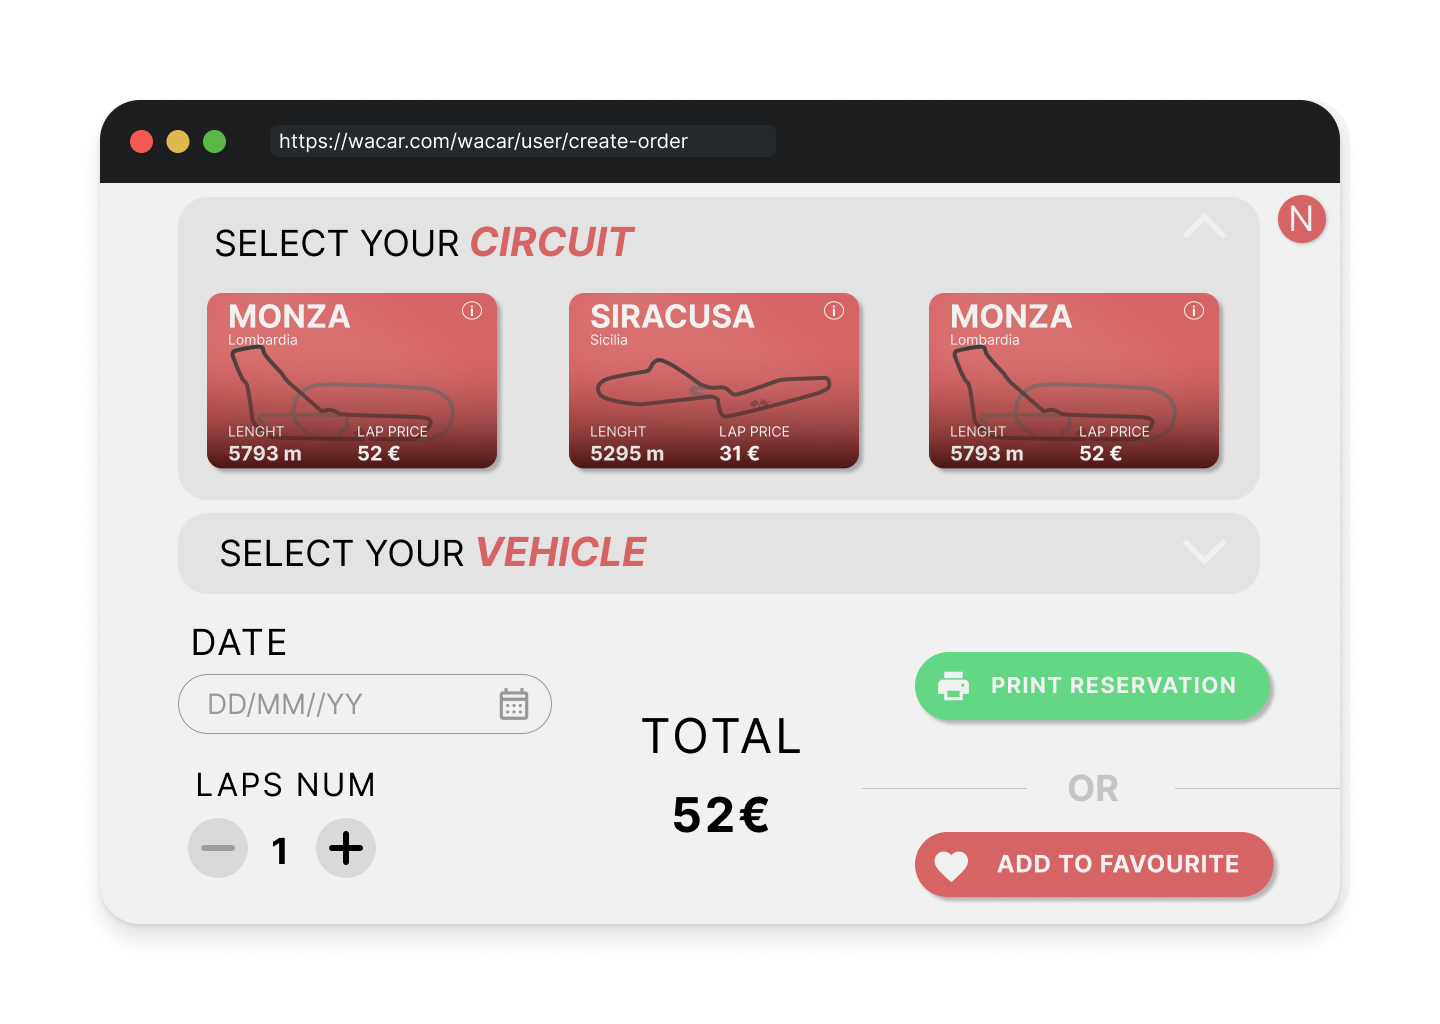
\includegraphics[scale=0.3]{./mockup/order_page_all_in_one.png}
	\captionof{figure}{WACAR order page}
	\label{ERSchema}
\end{center}